\documentclass[a4paper]{article}

%% Language and font encodings
\usepackage[english]{babel}
\usepackage[utf8x]{inputenc}
\usepackage[T1]{fontenc}
\usepackage{caption}
\usepackage{subcaption}

%% Sets page size and margins
\usepackage[a4paper,top=3cm,bottom=2cm,left=3cm,right=3cm,marginparwidth=1.75cm]{geometry}

%% Useful packages
\usepackage{amsmath}
\usepackage{graphicx}
\usepackage[colorinlistoftodos]{todonotes}
\usepackage{lipsum}

\title{Your Paper}
\author{You}

\begin{document}

\section{Appendix}

\subsection{Personae}


\begin{figure}[th]
  \centering
  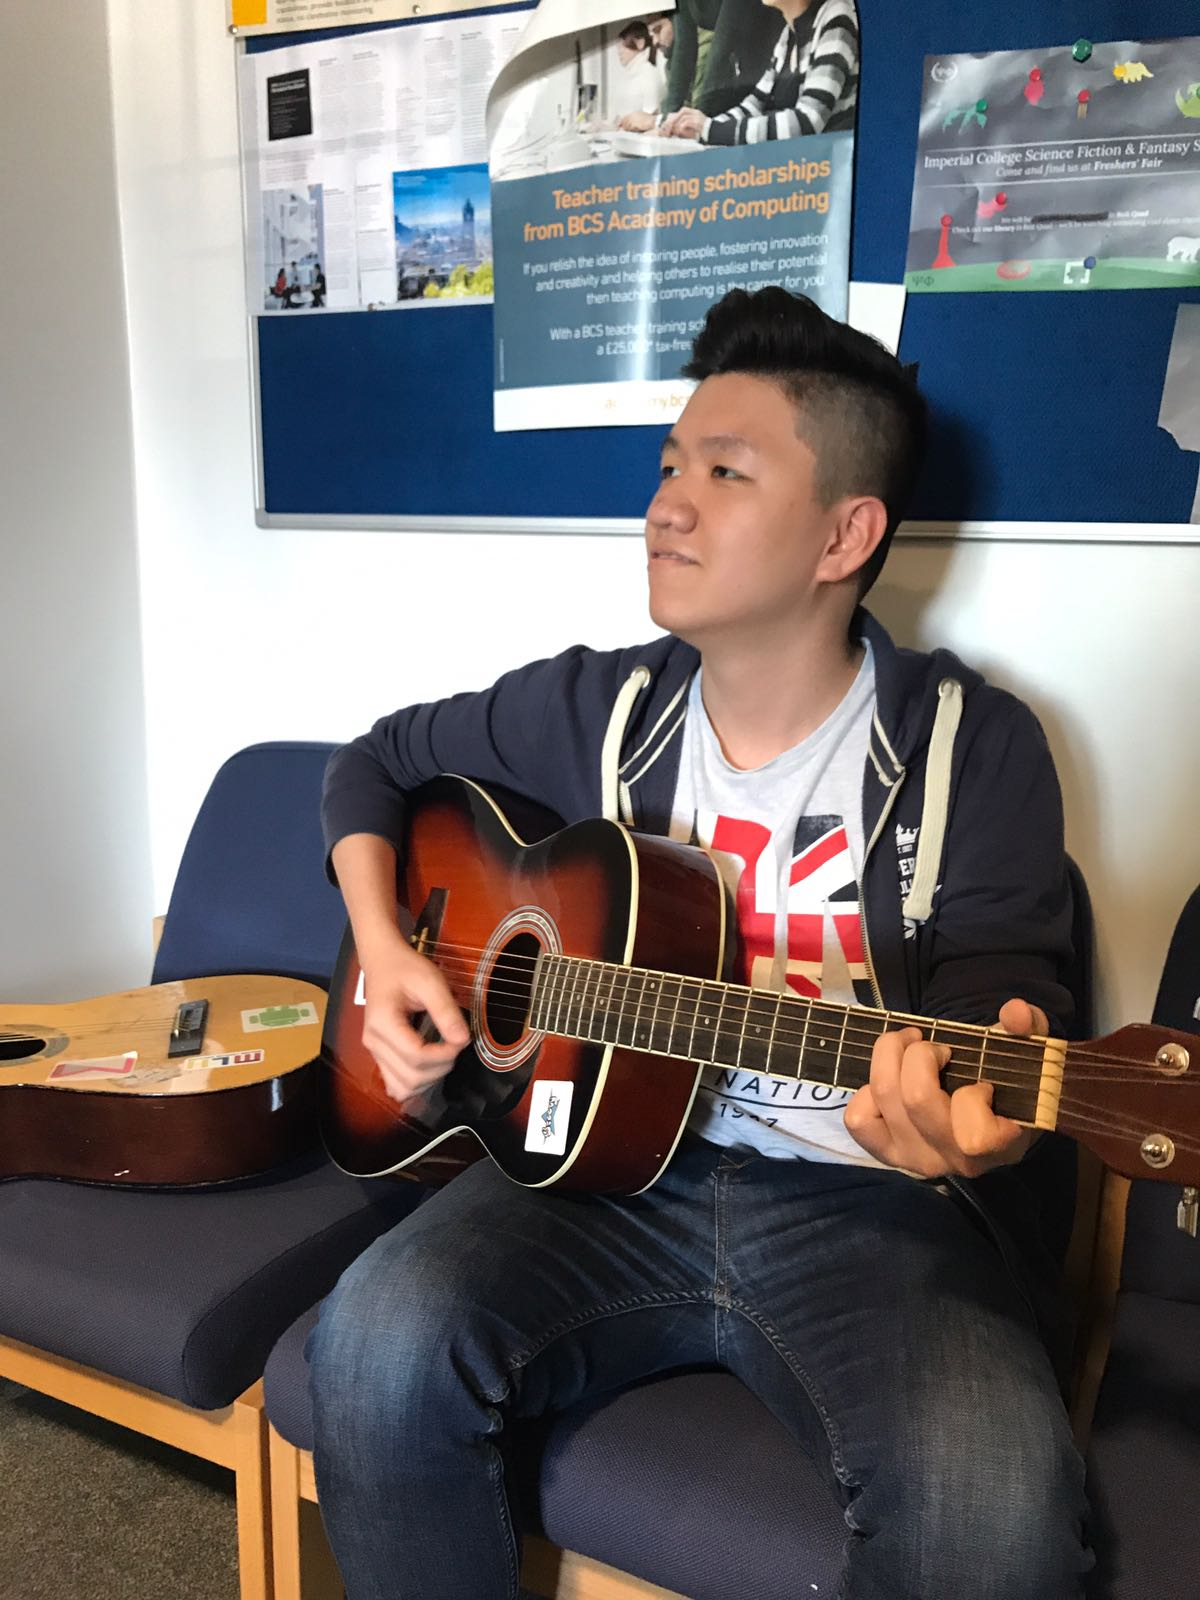
\includegraphics[width=.35\linewidth]{Max_2.jpeg}
  \caption{Max}
  \label{fig:Max}
\end{figure}

\begin{figure}[th]
  \centering
  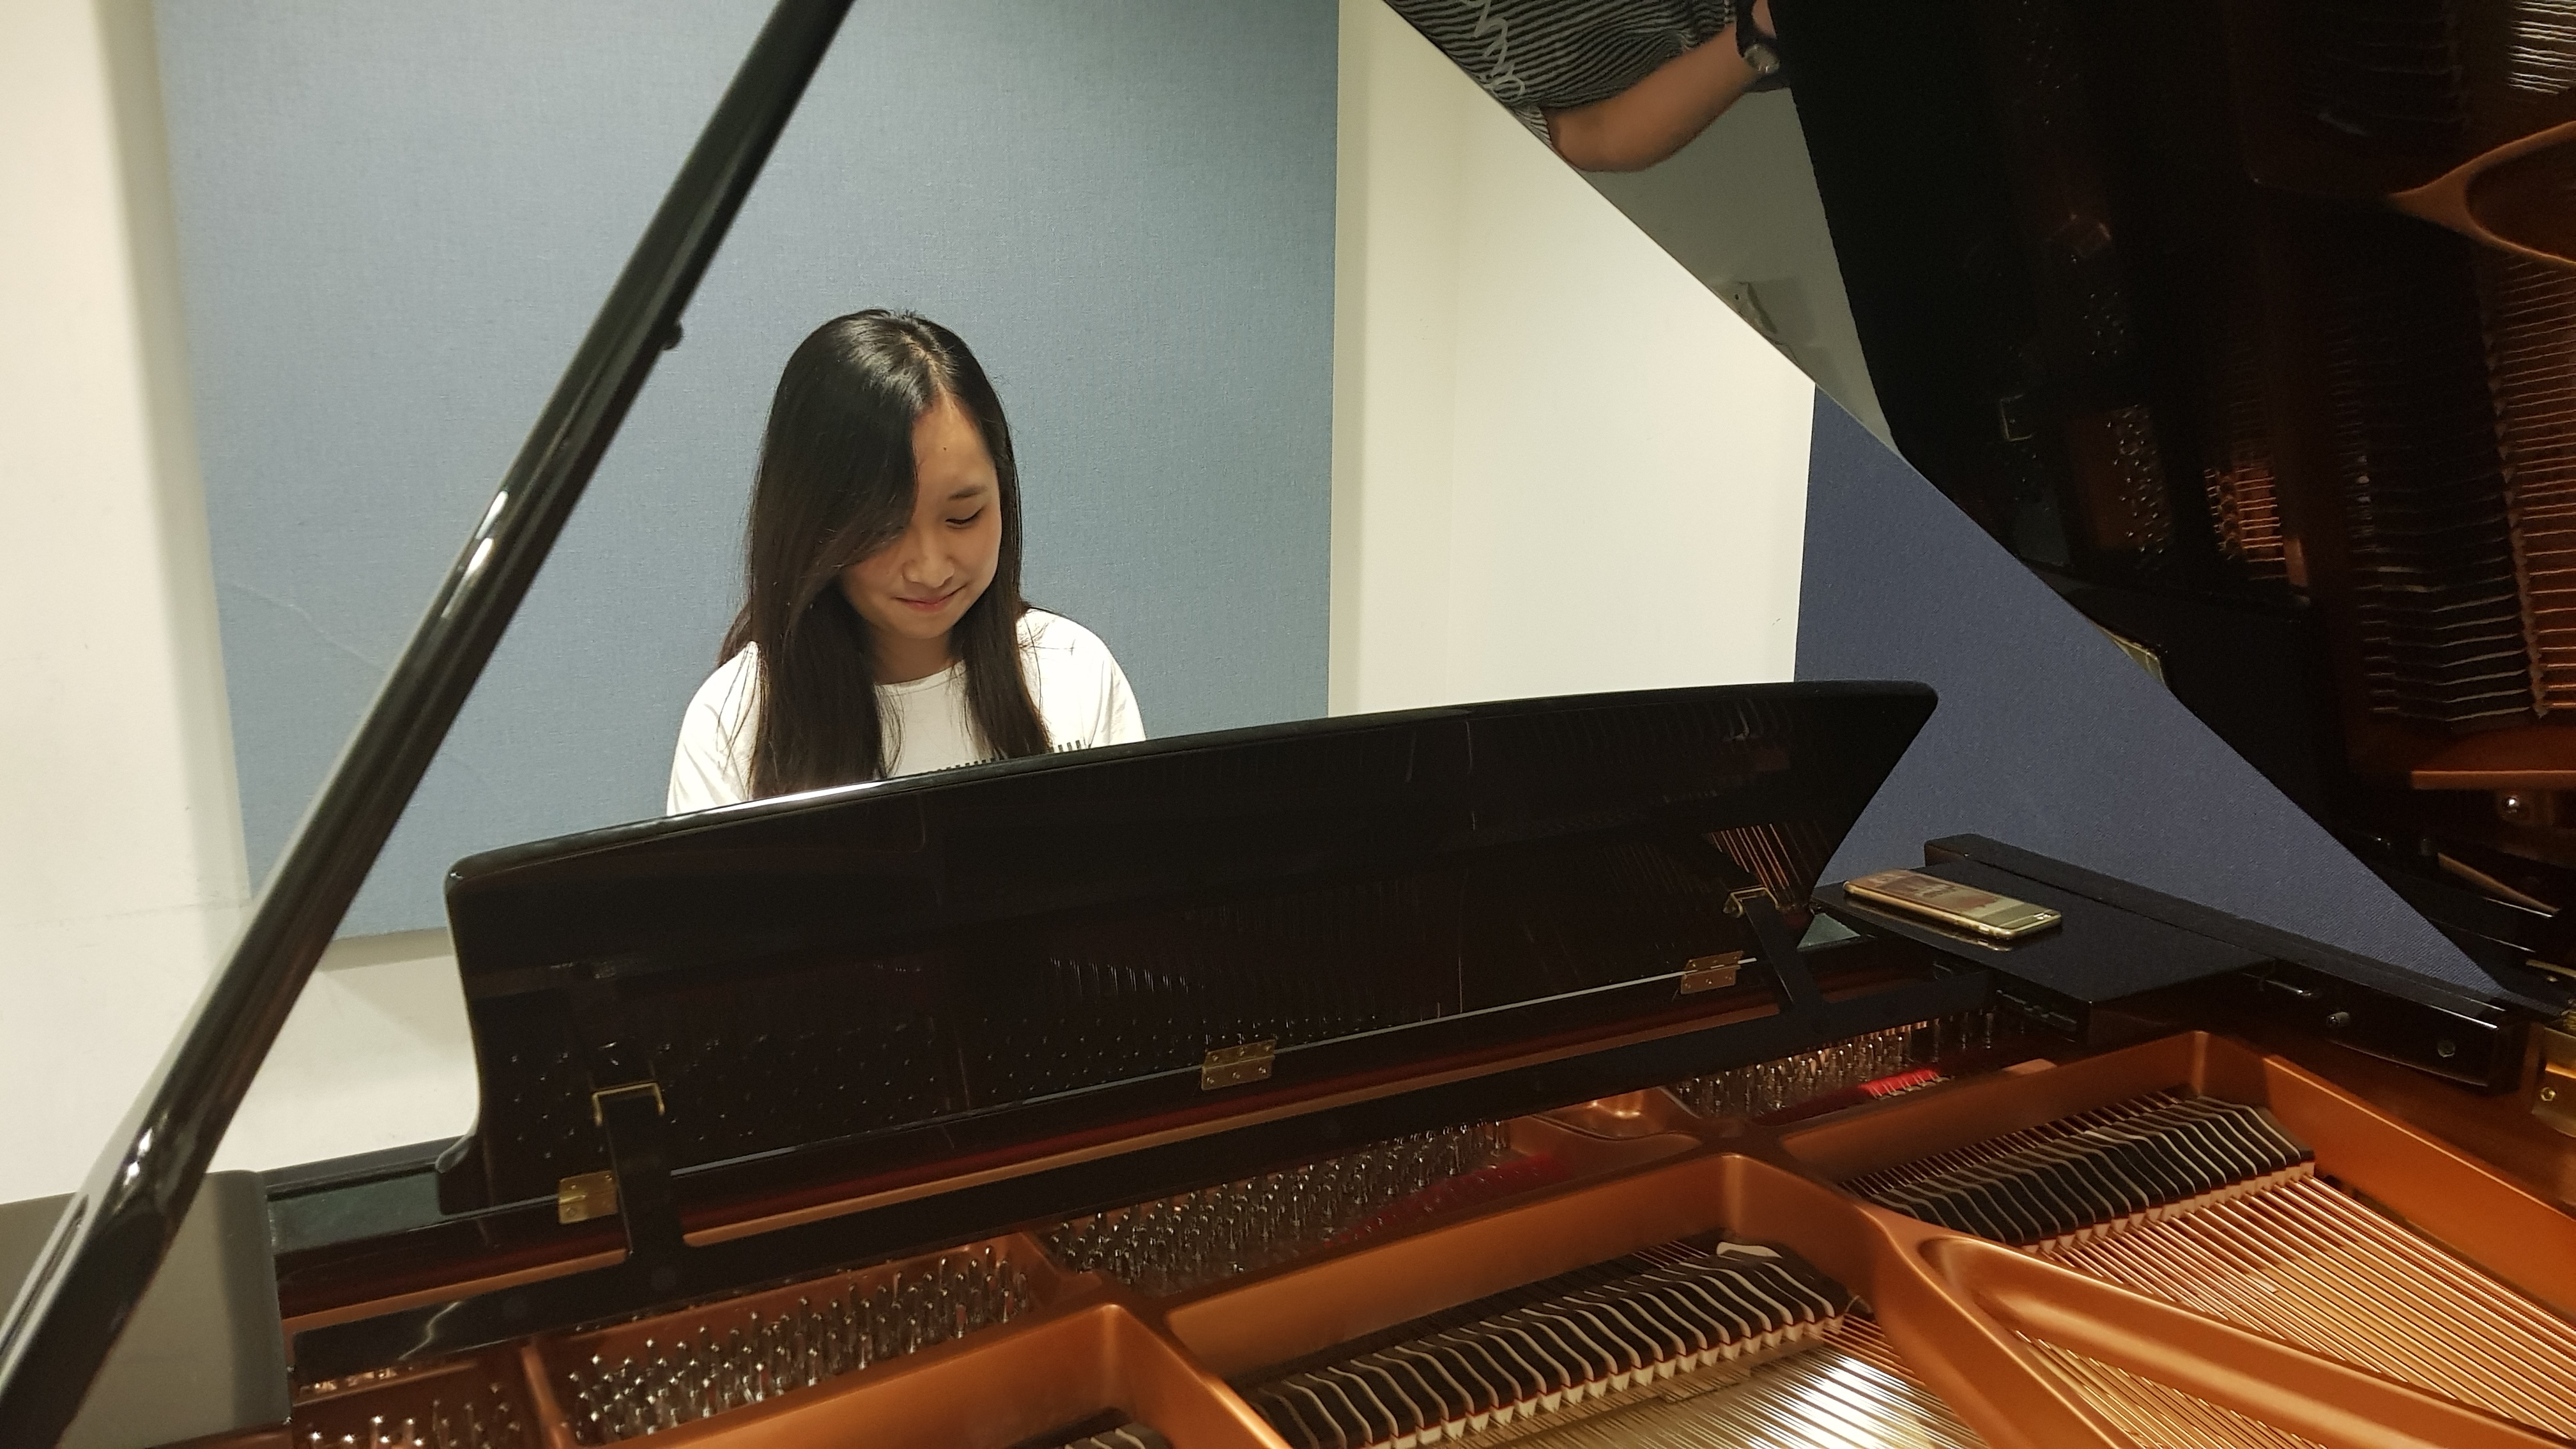
\includegraphics[width=.5\linewidth]{Kelly_1.jpeg}
  \caption{Kelly}
  \label{fig:kelly}
\end{figure}

\begin{table}[ht]
\centering
\begin{tabular}{l|r}
Kelly & Max \\\hline
Age: 23 & Age: 21 \\
Instrument: Piano/Keyboard & Instrument: Guitar
\end{tabular}
\end{table}

\clearpage

\begin{figure}[th]
  \centering
  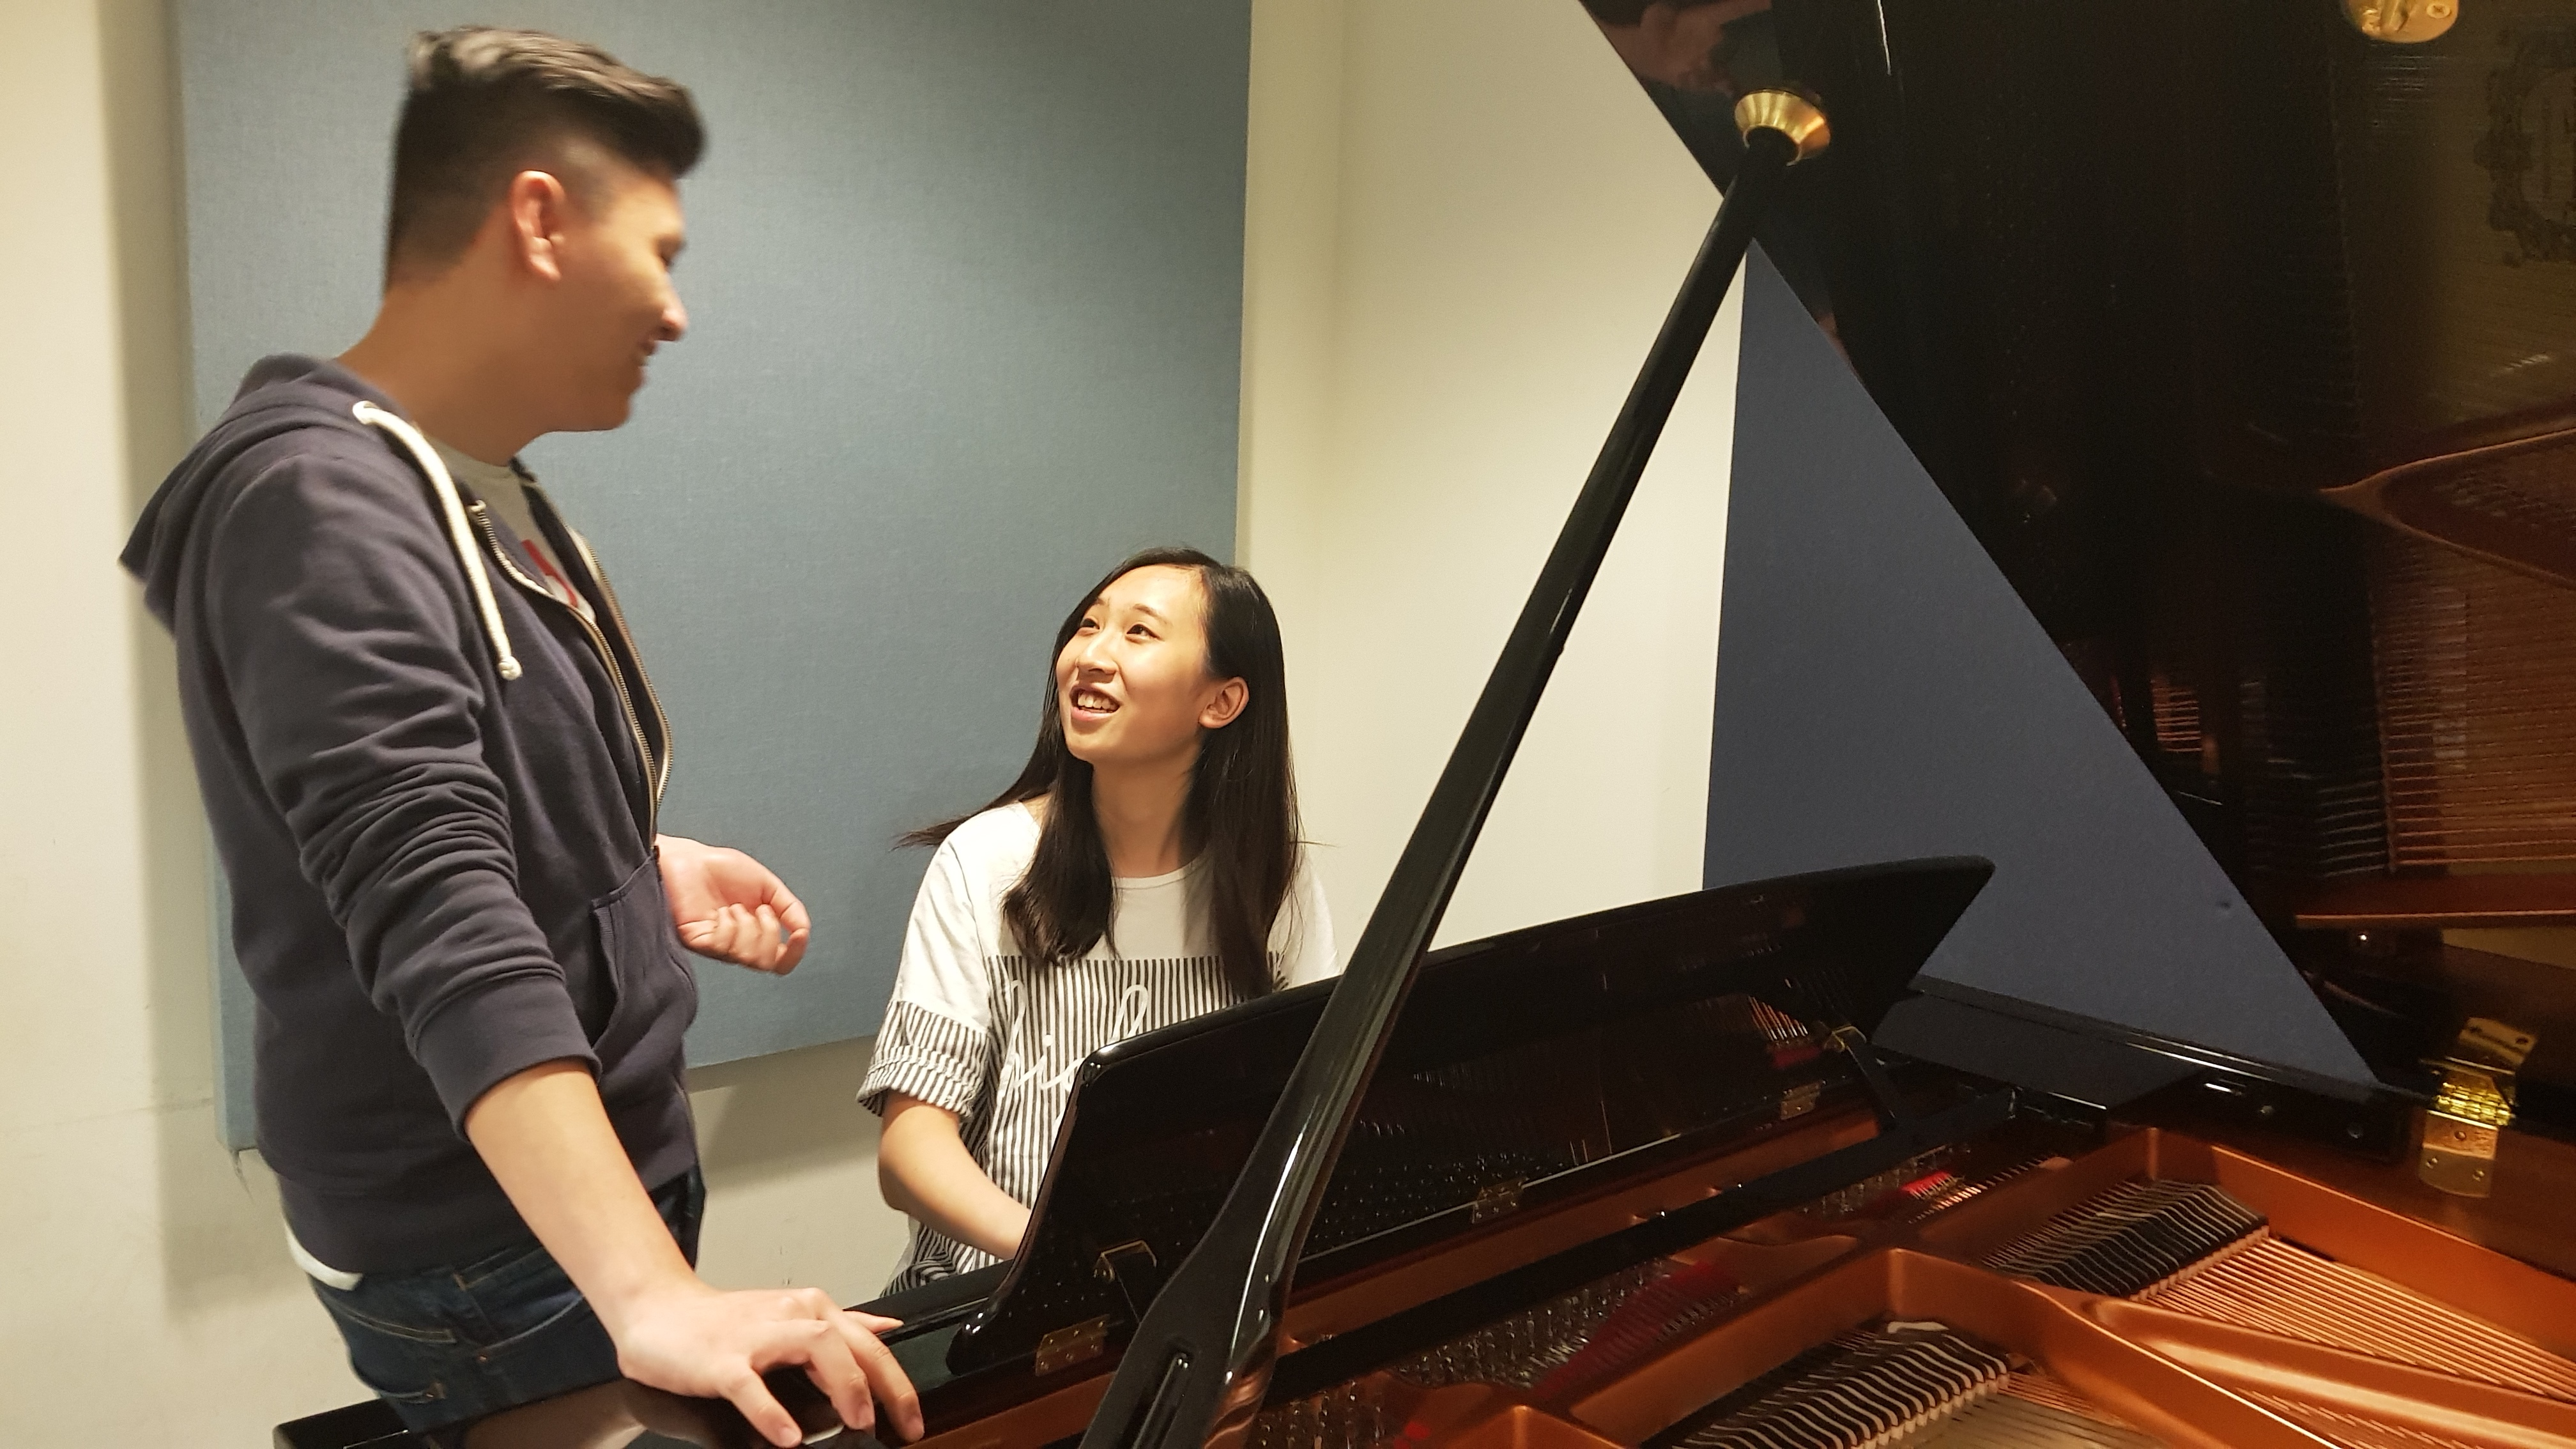
\includegraphics[width=.5\linewidth]{Collab_1.jpeg}
  \caption{Kelly and Max collaborating}
  \label{fig:collab}
\end{figure}


Max and Kelly are students of Imperial College and are participating in the student musical. They are collaborating to compose music for the musical.


\subsection{Existing work flow of collaborating composers}
Currently, Max and Kelly would plan an initial meet-up to discuss about the song. One of them would then transcribe the initial idea and send the music file via email to the other. Subsequent modifications would be made locally and then sent as a separate file, probably appended with its version number. \\
\\ 
Other messenging platforms like Whatsapp would be used to organise meetups or to make comments on the bar or to send annotated images to each other. \\
\\
At the end of the day, it is more often than not a huge mess of different files with non-standardised version names and feedback over different feedback channels which makes the changes really messy and hard to keep track of.


\begin{figure}[th]
\centering
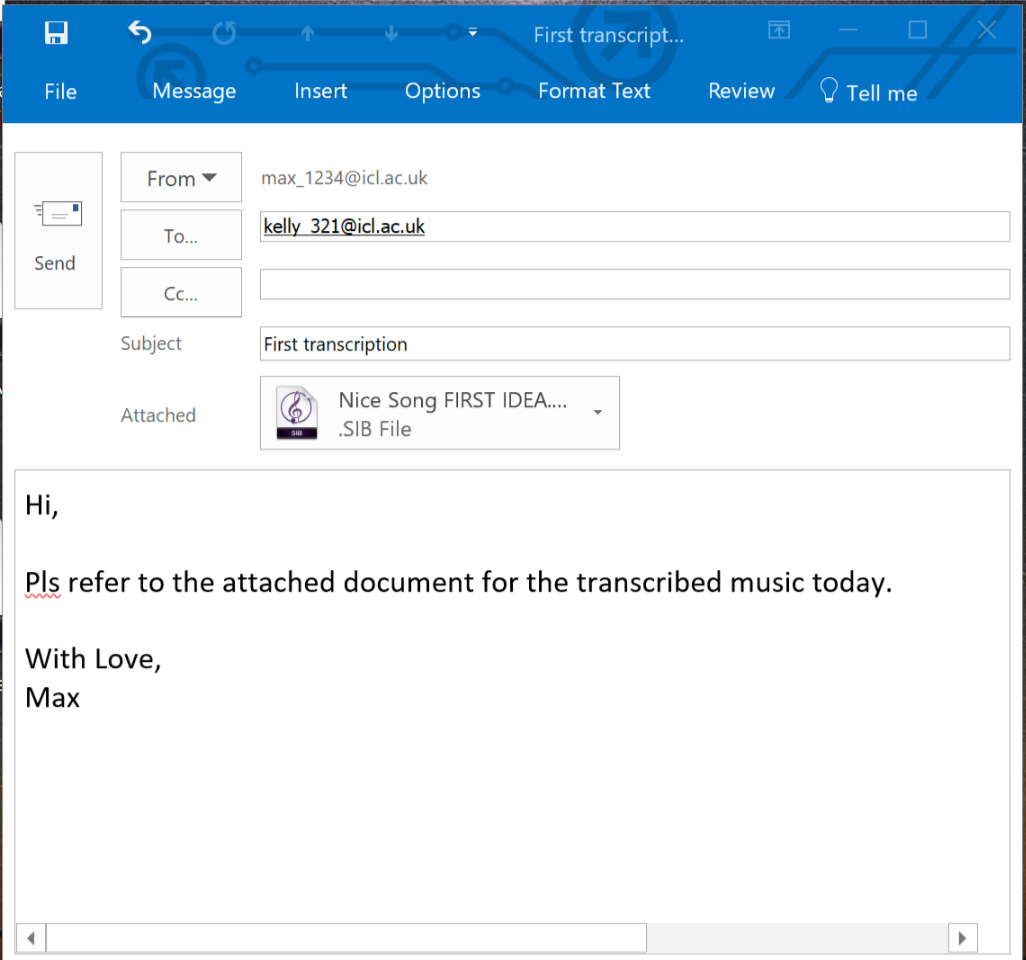
\includegraphics[width=0.75\textwidth]{Email.png}
\caption{\label{fig:email}Music notation files generally sent via email.}
\end{figure}

\begin{figure}[th]
\centering
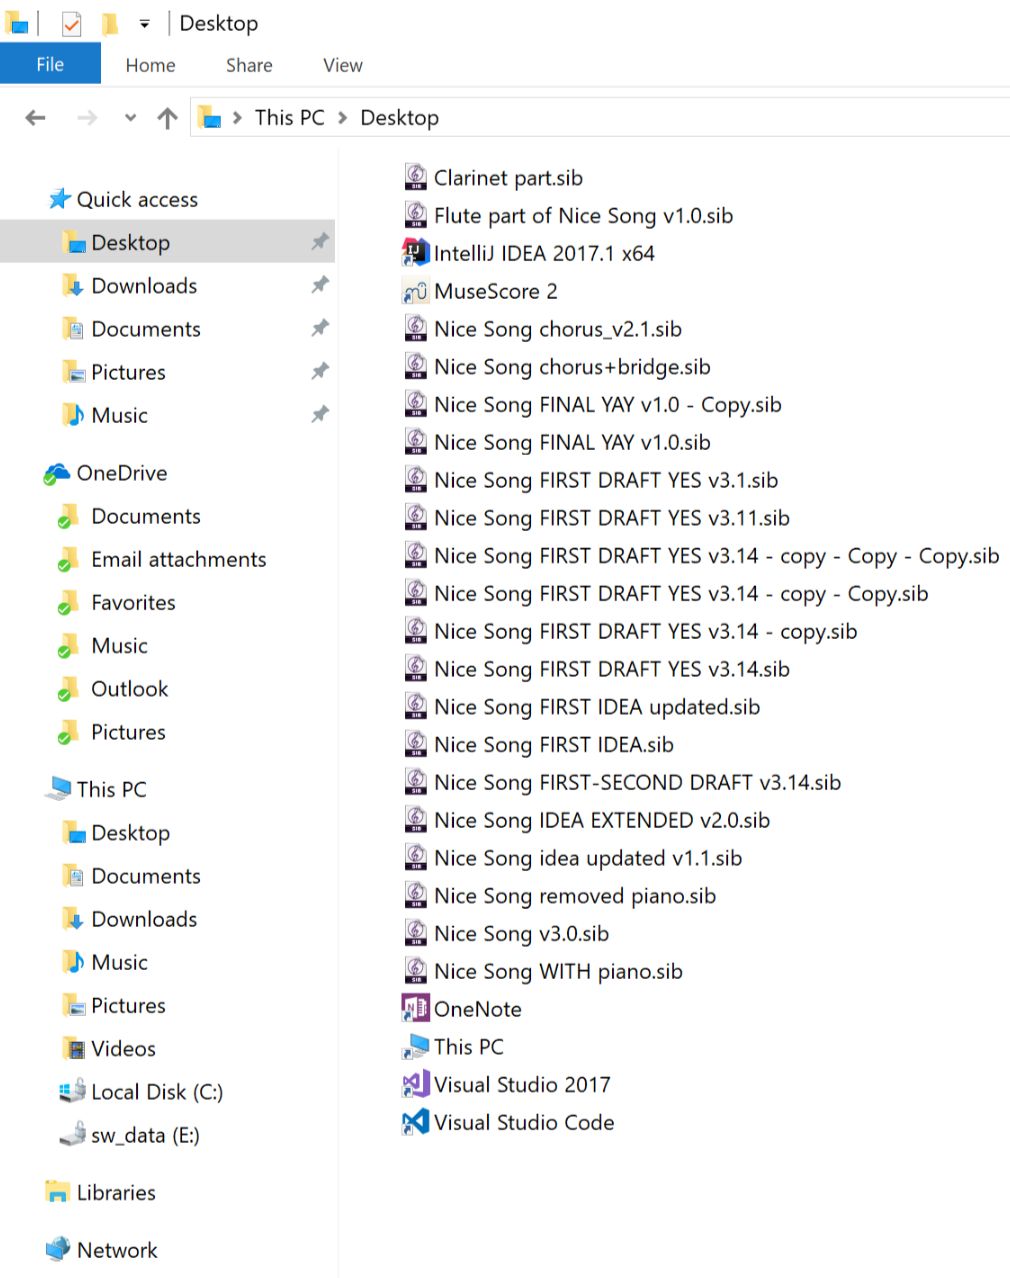
\includegraphics[width=0.7\textwidth]{Desktop_Folder.png}
\caption{\label{fig:desktop}Multiple revisions and edits leads to multiple versions of same composition.}
\end{figure}

\begin{figure}[th]
\centering
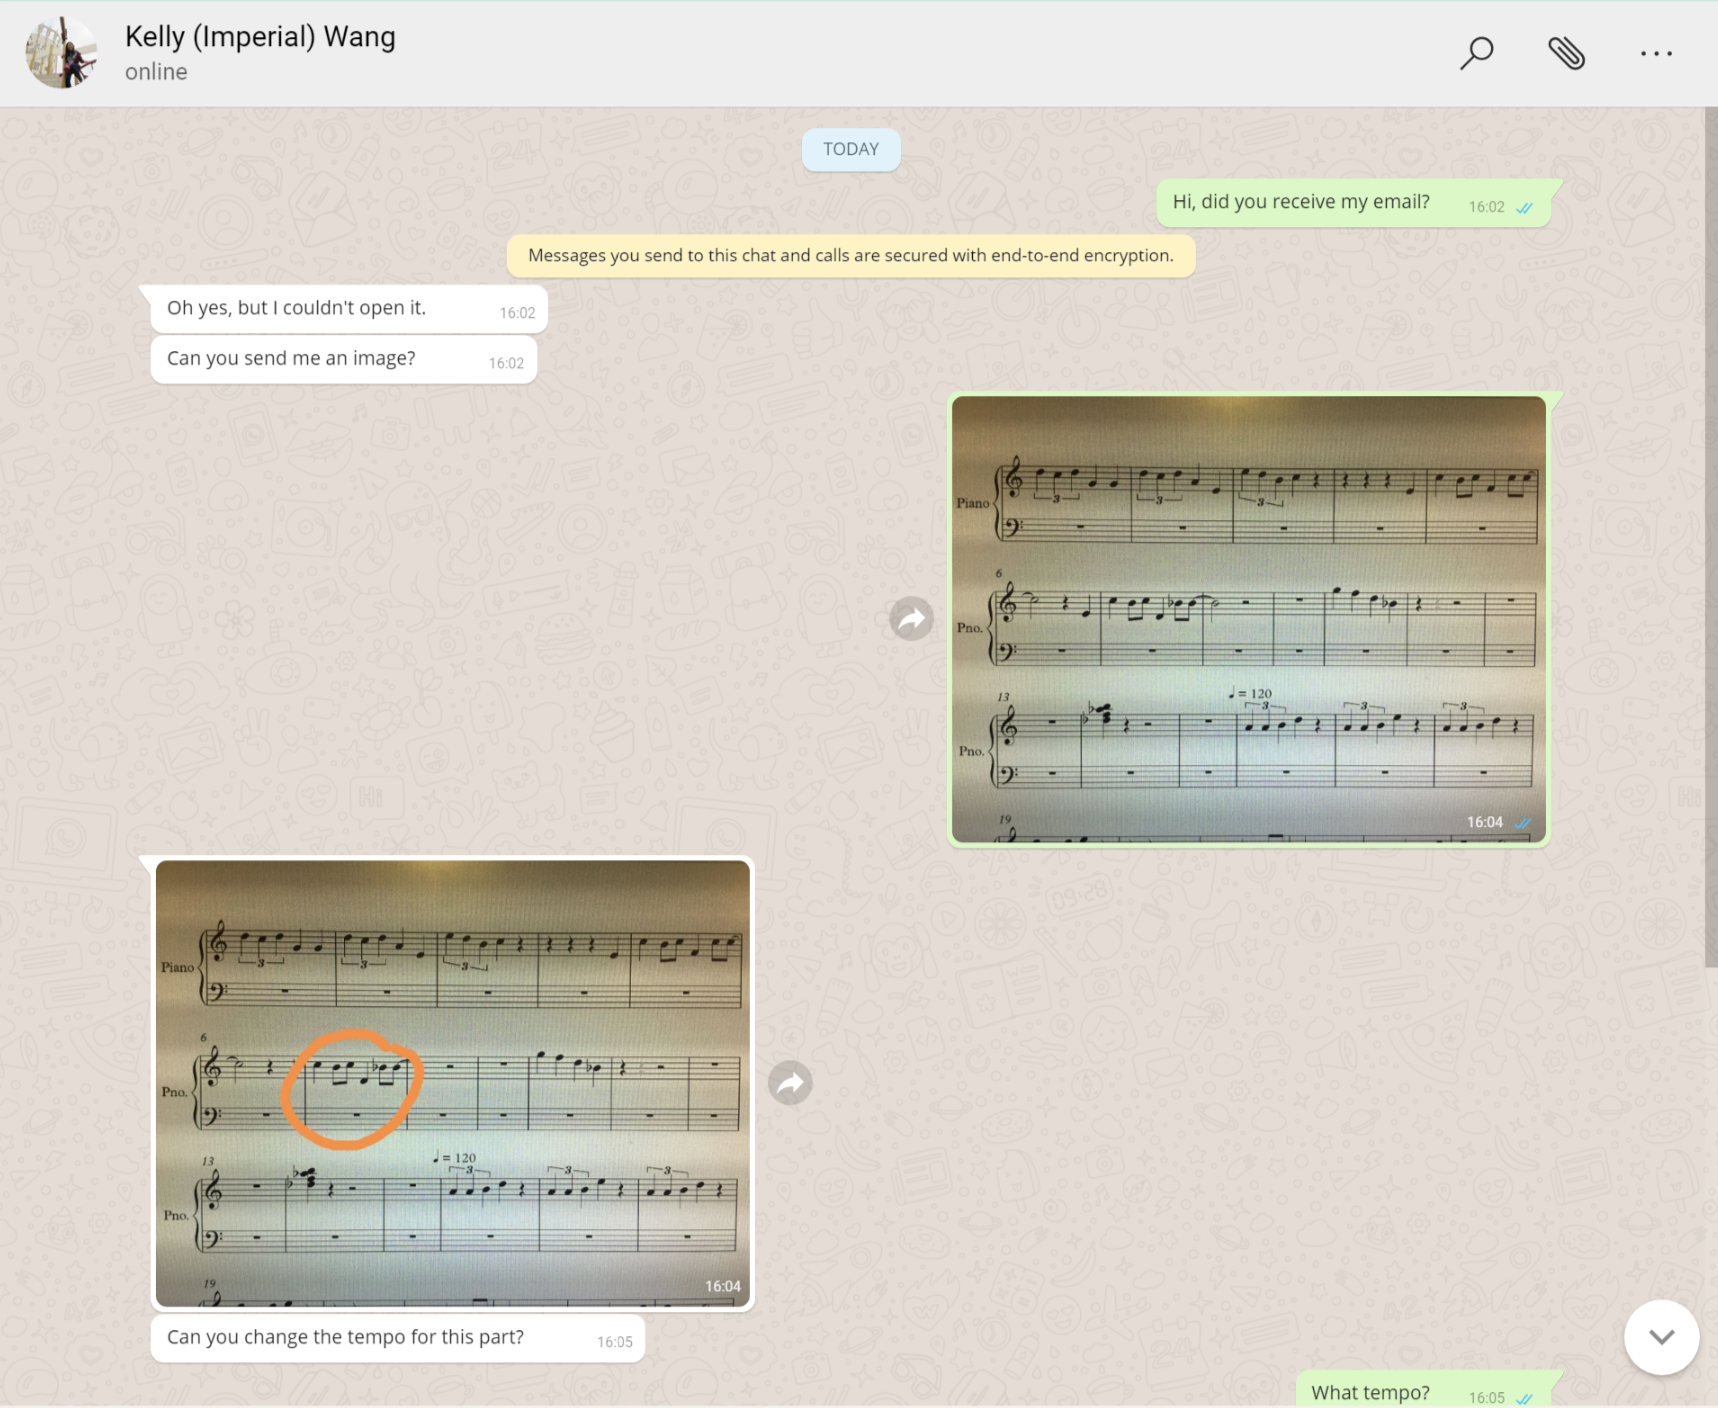
\includegraphics[width=0.75\textwidth]{Whatsapp1.png}
\caption{\label{fig:wa}Other platforms like Whatsapp messenger may be used to convey changes.}
\end{figure}

\subsection{Insights}
The collaboration process is very fragmented, multiple different platforms are used (email, Whatsapp, possibly others). Feedback channels are also fragmented, Max and Kelly have to sieve through all the email exchanges and possibly messenger conversations to look for comments on the composition, that could be in text form, audio form, or even images.\\
\\
Furthermore, it is difficult for Max and Kelly to talk about a specific change in a specific version, there is no notion of version control to pinpoint a specific change in the composition.

\end{document}